\section{A PINN para Solução de EDOs}

\begin{frame}{Estrutura da Rede Neural utilizada}
  A rede neural utilizada consiste em 5 camadas com a função de ativação tangente hiperbólica $(\tanh)$ entre elas.

  \begin{itemize}
    \item Entrada: $x = t$;
    \item camada linear 1: 32 neurônios;
    \item camada linear 2: 32 neurônios;
    \item camada linear 3: 32 neurônios;
    \item camada linear 4: 32 neurônios;
    \item saída: $\mathbf{y} = [h_1, h_2]$.
  \end{itemize}

  Totalizando $32+32+32+32+2=130$ neurônios.
\end{frame}

\begin{frame}{Entendendo a função \textit{loss} utilizada}
  A função \textit{loss} utilizada combina o erro baseado nas equações diferenciais com o erro de dados simulados.

  \begin{equation}
    \mathcal{L} = w_1 \cdot \mathcal{L}_{\text{EDO}} + w_2 \cdot \mathcal{L}_{\text{IC}} + w_3 \cdot \mathcal{L}_{\text{data}}
  \end{equation}
  onde:
  \begin{itemize}
    \item $w_1, w_2, w_3$: pesos para o cálculo da \textit{loss};
    \item $\mathcal{L}_{\text{EDO}}$: erro das equações diferenciais;
    \item $\mathcal{L}_{\text{IC}}$: erro das condições iniciais;
    \item $\mathcal{L}_{\text{data}}$: erro dos dados;
    \item $\mathcal{L}$: erro total.
  \end{itemize}
\end{frame}

\begin{frame}
  \begin{figure}
    \centering
    \resizebox{\textwidth}{!}{% Graphic for TeX using PGF
% Title: /home/silas/Downloads/prh-35.1/LaTeX/common/figures/pinn-diagram.dia
% Creator: Dia v0.97+git
% CreationDate: Tue Dec  3 14:40:09 2024
% For: silas
% \usepackage{tikz}
% The following commands are not supported in PSTricks at present
% We define them conditionally, so when they are implemented,
% this pgf file will use them.
\ifx\du\undefined
  \newlength{\du}
\fi
\setlength{\du}{15\unitlength}
\begin{tikzpicture}[even odd rule]
  \pgftransformxscale{1.000000}
  \pgftransformyscale{-1.000000}
  \definecolor{dialinecolor}{rgb}{0.000000, 0.000000, 0.000000}
  \pgfsetstrokecolor{dialinecolor}
  \pgfsetstrokeopacity{1.000000}
  \definecolor{diafillcolor}{rgb}{1.000000, 1.000000, 1.000000}
  \pgfsetfillcolor{diafillcolor}
  \pgfsetfillopacity{1.000000}
  \pgfsetlinewidth{0.100000\du}
  \pgfsetdash{{0.300000\du}{0.300000\du}}{0\du}
  \pgfsetmiterjoin
  {\pgfsetcornersarced{\pgfpoint{0.500000\du}{0.500000\du}}\definecolor{diafillcolor}{rgb}{1.000000, 1.000000, 1.000000}
    \pgfsetfillcolor{diafillcolor}
    \pgfsetfillopacity{0.000000}
    \fill (34.000000\du,14.000000\du)--(34.000000\du,21.000000\du)--(38.000000\du,21.000000\du)--(38.000000\du,14.000000\du)--cycle;
  }{\pgfsetcornersarced{\pgfpoint{0.500000\du}{0.500000\du}}\definecolor{dialinecolor}{rgb}{0.000000, 0.000000, 0.000000}
    \pgfsetstrokecolor{dialinecolor}
    \pgfsetstrokeopacity{1.000000}
    \draw (34.000000\du,14.000000\du)--(34.000000\du,21.000000\du)--(38.000000\du,21.000000\du)--(38.000000\du,14.000000\du)--cycle;
  }% setfont left to latex
  \definecolor{dialinecolor}{rgb}{0.000000, 0.000000, 0.000000}
  \pgfsetstrokecolor{dialinecolor}
  \pgfsetstrokeopacity{1.000000}
  \definecolor{diafillcolor}{rgb}{0.000000, 0.000000, 0.000000}
  \pgfsetfillcolor{diafillcolor}
  \pgfsetfillopacity{1.000000}
  \node[anchor=base,inner sep=0pt, outer sep=0pt,color=dialinecolor] at (36.000000\du,17.691509\du){};
  \pgfsetlinewidth{0.100000\du}
  \pgfsetdash{{0.300000\du}{0.300000\du}}{0\du}
  \pgfsetmiterjoin
  {\pgfsetcornersarced{\pgfpoint{0.500000\du}{0.500000\du}}\definecolor{diafillcolor}{rgb}{1.000000, 1.000000, 1.000000}
    \pgfsetfillcolor{diafillcolor}
    \pgfsetfillopacity{0.000000}
    \fill (15.000000\du,14.000000\du)--(15.000000\du,27.000000\du)--(32.000000\du,27.000000\du)--(32.000000\du,14.000000\du)--cycle;
  }{\pgfsetcornersarced{\pgfpoint{0.500000\du}{0.500000\du}}\definecolor{dialinecolor}{rgb}{0.000000, 0.000000, 0.000000}
    \pgfsetstrokecolor{dialinecolor}
    \pgfsetstrokeopacity{1.000000}
    \draw (15.000000\du,14.000000\du)--(15.000000\du,27.000000\du)--(32.000000\du,27.000000\du)--(32.000000\du,14.000000\du)--cycle;
  }% setfont left to latex
  \definecolor{dialinecolor}{rgb}{0.000000, 0.000000, 0.000000}
  \pgfsetstrokecolor{dialinecolor}
  \pgfsetstrokeopacity{1.000000}
  \definecolor{diafillcolor}{rgb}{0.000000, 0.000000, 0.000000}
  \pgfsetfillcolor{diafillcolor}
  \pgfsetfillopacity{1.000000}
  \node[anchor=base,inner sep=0pt, outer sep=0pt,color=dialinecolor] at (23.500000\du,20.691509\du){};
  \pgfsetlinewidth{0.100000\du}
  \pgfsetdash{}{0pt}
  \pgfsetmiterjoin
  \definecolor{diafillcolor}{rgb}{1.000000, 1.000000, 1.000000}
  \pgfsetfillcolor{diafillcolor}
  \pgfsetfillopacity{1.000000}
  \pgfpathellipse{\pgfpoint{16.500000\du}{20.500000\du}}{\pgfpoint{1.000000\du}{0\du}}{\pgfpoint{0\du}{1.000000\du}}
  \pgfusepath{fill}
  \definecolor{dialinecolor}{rgb}{0.000000, 0.000000, 0.000000}
  \pgfsetstrokecolor{dialinecolor}
  \pgfsetstrokeopacity{1.000000}
  \pgfpathellipse{\pgfpoint{16.500000\du}{20.500000\du}}{\pgfpoint{1.000000\du}{0\du}}{\pgfpoint{0\du}{1.000000\du}}
  \pgfusepath{stroke}
  % setfont left to latex
  \definecolor{dialinecolor}{rgb}{0.000000, 0.000000, 0.000000}
  \pgfsetstrokecolor{dialinecolor}
  \pgfsetstrokeopacity{1.000000}
  \definecolor{diafillcolor}{rgb}{0.000000, 0.000000, 0.000000}
  \pgfsetfillcolor{diafillcolor}
  \pgfsetfillopacity{1.000000}
  \node[anchor=base,inner sep=0pt, outer sep=0pt,color=dialinecolor] at (16.500000\du,20.694063\du){};
  \pgfsetlinewidth{0.100000\du}
  \pgfsetdash{}{0pt}
  \pgfsetmiterjoin
  \definecolor{diafillcolor}{rgb}{1.000000, 1.000000, 1.000000}
  \pgfsetfillcolor{diafillcolor}
  \pgfsetfillopacity{1.000000}
  \pgfpathellipse{\pgfpoint{21.000000\du}{16.000000\du}}{\pgfpoint{1.000000\du}{0\du}}{\pgfpoint{0\du}{1.000000\du}}
  \pgfusepath{fill}
  \definecolor{dialinecolor}{rgb}{0.000000, 0.000000, 0.000000}
  \pgfsetstrokecolor{dialinecolor}
  \pgfsetstrokeopacity{1.000000}
  \pgfpathellipse{\pgfpoint{21.000000\du}{16.000000\du}}{\pgfpoint{1.000000\du}{0\du}}{\pgfpoint{0\du}{1.000000\du}}
  \pgfusepath{stroke}
  % setfont left to latex
  \definecolor{dialinecolor}{rgb}{0.000000, 0.000000, 0.000000}
  \pgfsetstrokecolor{dialinecolor}
  \pgfsetstrokeopacity{1.000000}
  \definecolor{diafillcolor}{rgb}{0.000000, 0.000000, 0.000000}
  \pgfsetfillcolor{diafillcolor}
  \pgfsetfillopacity{1.000000}
  \node[anchor=base,inner sep=0pt, outer sep=0pt,color=dialinecolor] at (21.000000\du,16.194063\du){};
  \pgfsetlinewidth{0.100000\du}
  \pgfsetdash{}{0pt}
  \pgfsetmiterjoin
  \definecolor{diafillcolor}{rgb}{1.000000, 1.000000, 1.000000}
  \pgfsetfillcolor{diafillcolor}
  \pgfsetfillopacity{1.000000}
  \pgfpathellipse{\pgfpoint{21.000000\du}{19.000000\du}}{\pgfpoint{1.000000\du}{0\du}}{\pgfpoint{0\du}{1.000000\du}}
  \pgfusepath{fill}
  \definecolor{dialinecolor}{rgb}{0.000000, 0.000000, 0.000000}
  \pgfsetstrokecolor{dialinecolor}
  \pgfsetstrokeopacity{1.000000}
  \pgfpathellipse{\pgfpoint{21.000000\du}{19.000000\du}}{\pgfpoint{1.000000\du}{0\du}}{\pgfpoint{0\du}{1.000000\du}}
  \pgfusepath{stroke}
  % setfont left to latex
  \definecolor{dialinecolor}{rgb}{0.000000, 0.000000, 0.000000}
  \pgfsetstrokecolor{dialinecolor}
  \pgfsetstrokeopacity{1.000000}
  \definecolor{diafillcolor}{rgb}{0.000000, 0.000000, 0.000000}
  \pgfsetfillcolor{diafillcolor}
  \pgfsetfillopacity{1.000000}
  \node[anchor=base,inner sep=0pt, outer sep=0pt,color=dialinecolor] at (21.000000\du,19.194063\du){};
  \pgfsetlinewidth{0.100000\du}
  \pgfsetdash{}{0pt}
  \pgfsetmiterjoin
  \definecolor{diafillcolor}{rgb}{1.000000, 1.000000, 1.000000}
  \pgfsetfillcolor{diafillcolor}
  \pgfsetfillopacity{1.000000}
  \pgfpathellipse{\pgfpoint{21.000000\du}{25.000000\du}}{\pgfpoint{1.000000\du}{0\du}}{\pgfpoint{0\du}{1.000000\du}}
  \pgfusepath{fill}
  \definecolor{dialinecolor}{rgb}{0.000000, 0.000000, 0.000000}
  \pgfsetstrokecolor{dialinecolor}
  \pgfsetstrokeopacity{1.000000}
  \pgfpathellipse{\pgfpoint{21.000000\du}{25.000000\du}}{\pgfpoint{1.000000\du}{0\du}}{\pgfpoint{0\du}{1.000000\du}}
  \pgfusepath{stroke}
  % setfont left to latex
  \definecolor{dialinecolor}{rgb}{0.000000, 0.000000, 0.000000}
  \pgfsetstrokecolor{dialinecolor}
  \pgfsetstrokeopacity{1.000000}
  \definecolor{diafillcolor}{rgb}{0.000000, 0.000000, 0.000000}
  \pgfsetfillcolor{diafillcolor}
  \pgfsetfillopacity{1.000000}
  \node[anchor=base,inner sep=0pt, outer sep=0pt,color=dialinecolor] at (21.000000\du,25.194063\du){};
  \pgfsetlinewidth{0.100000\du}
  \pgfsetdash{}{0pt}
  \pgfsetmiterjoin
  \definecolor{diafillcolor}{rgb}{1.000000, 1.000000, 1.000000}
  \pgfsetfillcolor{diafillcolor}
  \pgfsetfillopacity{1.000000}
  \pgfpathellipse{\pgfpoint{25.500000\du}{16.000000\du}}{\pgfpoint{1.000000\du}{0\du}}{\pgfpoint{0\du}{1.000000\du}}
  \pgfusepath{fill}
  \definecolor{dialinecolor}{rgb}{0.000000, 0.000000, 0.000000}
  \pgfsetstrokecolor{dialinecolor}
  \pgfsetstrokeopacity{1.000000}
  \pgfpathellipse{\pgfpoint{25.500000\du}{16.000000\du}}{\pgfpoint{1.000000\du}{0\du}}{\pgfpoint{0\du}{1.000000\du}}
  \pgfusepath{stroke}
  % setfont left to latex
  \definecolor{dialinecolor}{rgb}{0.000000, 0.000000, 0.000000}
  \pgfsetstrokecolor{dialinecolor}
  \pgfsetstrokeopacity{1.000000}
  \definecolor{diafillcolor}{rgb}{0.000000, 0.000000, 0.000000}
  \pgfsetfillcolor{diafillcolor}
  \pgfsetfillopacity{1.000000}
  \node[anchor=base,inner sep=0pt, outer sep=0pt,color=dialinecolor] at (25.500000\du,16.194063\du){};
  \pgfsetlinewidth{0.100000\du}
  \pgfsetdash{}{0pt}
  \pgfsetmiterjoin
  \definecolor{diafillcolor}{rgb}{1.000000, 1.000000, 1.000000}
  \pgfsetfillcolor{diafillcolor}
  \pgfsetfillopacity{1.000000}
  \pgfpathellipse{\pgfpoint{25.500000\du}{19.000000\du}}{\pgfpoint{1.000000\du}{0\du}}{\pgfpoint{0\du}{1.000000\du}}
  \pgfusepath{fill}
  \definecolor{dialinecolor}{rgb}{0.000000, 0.000000, 0.000000}
  \pgfsetstrokecolor{dialinecolor}
  \pgfsetstrokeopacity{1.000000}
  \pgfpathellipse{\pgfpoint{25.500000\du}{19.000000\du}}{\pgfpoint{1.000000\du}{0\du}}{\pgfpoint{0\du}{1.000000\du}}
  \pgfusepath{stroke}
  % setfont left to latex
  \definecolor{dialinecolor}{rgb}{0.000000, 0.000000, 0.000000}
  \pgfsetstrokecolor{dialinecolor}
  \pgfsetstrokeopacity{1.000000}
  \definecolor{diafillcolor}{rgb}{0.000000, 0.000000, 0.000000}
  \pgfsetfillcolor{diafillcolor}
  \pgfsetfillopacity{1.000000}
  \node[anchor=base,inner sep=0pt, outer sep=0pt,color=dialinecolor] at (25.500000\du,19.194063\du){};
  \pgfsetlinewidth{0.100000\du}
  \pgfsetdash{}{0pt}
  \pgfsetmiterjoin
  \definecolor{diafillcolor}{rgb}{1.000000, 1.000000, 1.000000}
  \pgfsetfillcolor{diafillcolor}
  \pgfsetfillopacity{1.000000}
  \pgfpathellipse{\pgfpoint{25.500000\du}{25.000000\du}}{\pgfpoint{1.000000\du}{0\du}}{\pgfpoint{0\du}{1.000000\du}}
  \pgfusepath{fill}
  \definecolor{dialinecolor}{rgb}{0.000000, 0.000000, 0.000000}
  \pgfsetstrokecolor{dialinecolor}
  \pgfsetstrokeopacity{1.000000}
  \pgfpathellipse{\pgfpoint{25.500000\du}{25.000000\du}}{\pgfpoint{1.000000\du}{0\du}}{\pgfpoint{0\du}{1.000000\du}}
  \pgfusepath{stroke}
  % setfont left to latex
  \definecolor{dialinecolor}{rgb}{0.000000, 0.000000, 0.000000}
  \pgfsetstrokecolor{dialinecolor}
  \pgfsetstrokeopacity{1.000000}
  \definecolor{diafillcolor}{rgb}{0.000000, 0.000000, 0.000000}
  \pgfsetfillcolor{diafillcolor}
  \pgfsetfillopacity{1.000000}
  \node[anchor=base,inner sep=0pt, outer sep=0pt,color=dialinecolor] at (25.500000\du,25.194063\du){};
  \pgfsetlinewidth{0.100000\du}
  \pgfsetdash{}{0pt}
  \pgfsetmiterjoin
  \definecolor{diafillcolor}{rgb}{1.000000, 1.000000, 1.000000}
  \pgfsetfillcolor{diafillcolor}
  \pgfsetfillopacity{1.000000}
  \pgfpathellipse{\pgfpoint{30.000000\du}{19.000000\du}}{\pgfpoint{1.000000\du}{0\du}}{\pgfpoint{0\du}{1.000000\du}}
  \pgfusepath{fill}
  \definecolor{dialinecolor}{rgb}{0.000000, 0.000000, 0.000000}
  \pgfsetstrokecolor{dialinecolor}
  \pgfsetstrokeopacity{1.000000}
  \pgfpathellipse{\pgfpoint{30.000000\du}{19.000000\du}}{\pgfpoint{1.000000\du}{0\du}}{\pgfpoint{0\du}{1.000000\du}}
  \pgfusepath{stroke}
  % setfont left to latex
  \definecolor{dialinecolor}{rgb}{0.000000, 0.000000, 0.000000}
  \pgfsetstrokecolor{dialinecolor}
  \pgfsetstrokeopacity{1.000000}
  \definecolor{diafillcolor}{rgb}{0.000000, 0.000000, 0.000000}
  \pgfsetfillcolor{diafillcolor}
  \pgfsetfillopacity{1.000000}
  \node[anchor=base,inner sep=0pt, outer sep=0pt,color=dialinecolor] at (30.000000\du,19.194063\du){};
  \pgfsetlinewidth{0.100000\du}
  \pgfsetdash{}{0pt}
  \pgfsetmiterjoin
  \definecolor{diafillcolor}{rgb}{1.000000, 1.000000, 1.000000}
  \pgfsetfillcolor{diafillcolor}
  \pgfsetfillopacity{1.000000}
  \pgfpathellipse{\pgfpoint{30.000000\du}{22.000000\du}}{\pgfpoint{1.000000\du}{0\du}}{\pgfpoint{0\du}{1.000000\du}}
  \pgfusepath{fill}
  \definecolor{dialinecolor}{rgb}{0.000000, 0.000000, 0.000000}
  \pgfsetstrokecolor{dialinecolor}
  \pgfsetstrokeopacity{1.000000}
  \pgfpathellipse{\pgfpoint{30.000000\du}{22.000000\du}}{\pgfpoint{1.000000\du}{0\du}}{\pgfpoint{0\du}{1.000000\du}}
  \pgfusepath{stroke}
  % setfont left to latex
  \definecolor{dialinecolor}{rgb}{0.000000, 0.000000, 0.000000}
  \pgfsetstrokecolor{dialinecolor}
  \pgfsetstrokeopacity{1.000000}
  \definecolor{diafillcolor}{rgb}{0.000000, 0.000000, 0.000000}
  \pgfsetfillcolor{diafillcolor}
  \pgfsetfillopacity{1.000000}
  \node[anchor=base,inner sep=0pt, outer sep=0pt,color=dialinecolor] at (30.000000\du,22.194063\du){};
  \pgfsetlinewidth{0.100000\du}
  \pgfsetdash{}{0pt}
  \pgfsetbuttcap
  {
    \definecolor{diafillcolor}{rgb}{0.000000, 0.000000, 0.000000}
    \pgfsetfillcolor{diafillcolor}
    \pgfsetfillopacity{1.000000}
    % was here!!!
    \pgfsetarrowsend{stealth}
    \definecolor{dialinecolor}{rgb}{0.000000, 0.000000, 0.000000}
    \pgfsetstrokecolor{dialinecolor}
    \pgfsetstrokeopacity{1.000000}
    \draw (17.500000\du,20.500000\du)--(20.000000\du,19.000000\du);
  }
  \pgfsetlinewidth{0.100000\du}
  \pgfsetdash{}{0pt}
  \pgfsetbuttcap
  {
    \definecolor{diafillcolor}{rgb}{0.000000, 0.000000, 0.000000}
    \pgfsetfillcolor{diafillcolor}
    \pgfsetfillopacity{1.000000}
    % was here!!!
    \pgfsetarrowsend{stealth}
    \definecolor{dialinecolor}{rgb}{0.000000, 0.000000, 0.000000}
    \pgfsetstrokecolor{dialinecolor}
    \pgfsetstrokeopacity{1.000000}
    \draw (17.500000\du,20.500000\du)--(20.000000\du,25.000000\du);
  }
  \pgfsetlinewidth{0.100000\du}
  \pgfsetdash{}{0pt}
  \pgfsetbuttcap
  {
    \definecolor{diafillcolor}{rgb}{0.000000, 0.000000, 0.000000}
    \pgfsetfillcolor{diafillcolor}
    \pgfsetfillopacity{1.000000}
    % was here!!!
    \pgfsetarrowsend{stealth}
    \definecolor{dialinecolor}{rgb}{0.000000, 0.000000, 0.000000}
    \pgfsetstrokecolor{dialinecolor}
    \pgfsetstrokeopacity{1.000000}
    \draw (17.500000\du,20.500000\du)--(20.000000\du,16.000000\du);
  }
  \pgfsetlinewidth{0.100000\du}
  \pgfsetdash{}{0pt}
  \pgfsetbuttcap
  {
    \definecolor{diafillcolor}{rgb}{0.000000, 0.000000, 0.000000}
    \pgfsetfillcolor{diafillcolor}
    \pgfsetfillopacity{1.000000}
    % was here!!!
    \pgfsetarrowsend{stealth}
    \definecolor{dialinecolor}{rgb}{0.000000, 0.000000, 0.000000}
    \pgfsetstrokecolor{dialinecolor}
    \pgfsetstrokeopacity{1.000000}
    \draw (26.500000\du,16.000000\du)--(29.000000\du,19.000000\du);
  }
  \pgfsetlinewidth{0.100000\du}
  \pgfsetdash{}{0pt}
  \pgfsetbuttcap
  {
    \definecolor{diafillcolor}{rgb}{0.000000, 0.000000, 0.000000}
    \pgfsetfillcolor{diafillcolor}
    \pgfsetfillopacity{1.000000}
    % was here!!!
    \pgfsetarrowsend{stealth}
    \definecolor{dialinecolor}{rgb}{0.000000, 0.000000, 0.000000}
    \pgfsetstrokecolor{dialinecolor}
    \pgfsetstrokeopacity{1.000000}
    \draw (26.500000\du,16.000000\du)--(29.000000\du,22.000000\du);
  }
  \pgfsetlinewidth{0.100000\du}
  \pgfsetdash{}{0pt}
  \pgfsetbuttcap
  {
    \definecolor{diafillcolor}{rgb}{0.000000, 0.000000, 0.000000}
    \pgfsetfillcolor{diafillcolor}
    \pgfsetfillopacity{1.000000}
    % was here!!!
    \pgfsetarrowsend{stealth}
    \definecolor{dialinecolor}{rgb}{0.000000, 0.000000, 0.000000}
    \pgfsetstrokecolor{dialinecolor}
    \pgfsetstrokeopacity{1.000000}
    \draw (26.500000\du,19.000000\du)--(29.000000\du,19.000000\du);
  }
  \pgfsetlinewidth{0.100000\du}
  \pgfsetdash{}{0pt}
  \pgfsetbuttcap
  {
    \definecolor{diafillcolor}{rgb}{0.000000, 0.000000, 0.000000}
    \pgfsetfillcolor{diafillcolor}
    \pgfsetfillopacity{1.000000}
    % was here!!!
    \pgfsetarrowsend{stealth}
    \definecolor{dialinecolor}{rgb}{0.000000, 0.000000, 0.000000}
    \pgfsetstrokecolor{dialinecolor}
    \pgfsetstrokeopacity{1.000000}
    \draw (26.500000\du,19.000000\du)--(29.000000\du,22.000000\du);
  }
  \pgfsetlinewidth{0.100000\du}
  \pgfsetdash{}{0pt}
  \pgfsetbuttcap
  {
    \definecolor{diafillcolor}{rgb}{0.000000, 0.000000, 0.000000}
    \pgfsetfillcolor{diafillcolor}
    \pgfsetfillopacity{1.000000}
    % was here!!!
    \pgfsetarrowsend{stealth}
    \definecolor{dialinecolor}{rgb}{0.000000, 0.000000, 0.000000}
    \pgfsetstrokecolor{dialinecolor}
    \pgfsetstrokeopacity{1.000000}
    \draw (26.500000\du,25.000000\du)--(29.000000\du,22.000000\du);
  }
  \pgfsetlinewidth{0.100000\du}
  \pgfsetdash{}{0pt}
  \pgfsetbuttcap
  {
    \definecolor{diafillcolor}{rgb}{0.000000, 0.000000, 0.000000}
    \pgfsetfillcolor{diafillcolor}
    \pgfsetfillopacity{1.000000}
    % was here!!!
    \pgfsetarrowsend{stealth}
    \definecolor{dialinecolor}{rgb}{0.000000, 0.000000, 0.000000}
    \pgfsetstrokecolor{dialinecolor}
    \pgfsetstrokeopacity{1.000000}
    \draw (26.500000\du,25.000000\du)--(29.000000\du,19.000000\du);
  }
  \pgfsetlinewidth{0.100000\du}
  \pgfsetdash{}{0pt}
  \pgfsetbuttcap
  {
    \definecolor{diafillcolor}{rgb}{0.000000, 0.000000, 0.000000}
    \pgfsetfillcolor{diafillcolor}
    \pgfsetfillopacity{1.000000}
    % was here!!!
    \pgfsetarrowsend{stealth}
    \definecolor{dialinecolor}{rgb}{0.000000, 0.000000, 0.000000}
    \pgfsetstrokecolor{dialinecolor}
    \pgfsetstrokeopacity{1.000000}
    \draw (22.000000\du,25.000000\du)--(24.500000\du,25.000000\du);
  }
  \pgfsetlinewidth{0.100000\du}
  \pgfsetdash{}{0pt}
  \pgfsetbuttcap
  {
    \definecolor{diafillcolor}{rgb}{0.000000, 0.000000, 0.000000}
    \pgfsetfillcolor{diafillcolor}
    \pgfsetfillopacity{1.000000}
    % was here!!!
    \pgfsetarrowsend{stealth}
    \definecolor{dialinecolor}{rgb}{0.000000, 0.000000, 0.000000}
    \pgfsetstrokecolor{dialinecolor}
    \pgfsetstrokeopacity{1.000000}
    \draw (22.000000\du,16.000000\du)--(24.500000\du,16.000000\du);
  }
  \pgfsetlinewidth{0.100000\du}
  \pgfsetdash{}{0pt}
  \pgfsetbuttcap
  {
    \definecolor{diafillcolor}{rgb}{0.000000, 0.000000, 0.000000}
    \pgfsetfillcolor{diafillcolor}
    \pgfsetfillopacity{1.000000}
    % was here!!!
    \pgfsetarrowsend{stealth}
    \definecolor{dialinecolor}{rgb}{0.000000, 0.000000, 0.000000}
    \pgfsetstrokecolor{dialinecolor}
    \pgfsetstrokeopacity{1.000000}
    \draw (22.000000\du,16.000000\du)--(24.500000\du,19.000000\du);
  }
  \pgfsetlinewidth{0.100000\du}
  \pgfsetdash{}{0pt}
  \pgfsetbuttcap
  {
    \definecolor{diafillcolor}{rgb}{0.000000, 0.000000, 0.000000}
    \pgfsetfillcolor{diafillcolor}
    \pgfsetfillopacity{1.000000}
    % was here!!!
    \pgfsetarrowsend{stealth}
    \definecolor{dialinecolor}{rgb}{0.000000, 0.000000, 0.000000}
    \pgfsetstrokecolor{dialinecolor}
    \pgfsetstrokeopacity{1.000000}
    \draw (22.000000\du,16.000000\du)--(24.500000\du,25.000000\du);
  }
  \pgfsetlinewidth{0.100000\du}
  \pgfsetdash{}{0pt}
  \pgfsetbuttcap
  {
    \definecolor{diafillcolor}{rgb}{0.000000, 0.000000, 0.000000}
    \pgfsetfillcolor{diafillcolor}
    \pgfsetfillopacity{1.000000}
    % was here!!!
    \pgfsetarrowsend{stealth}
    \definecolor{dialinecolor}{rgb}{0.000000, 0.000000, 0.000000}
    \pgfsetstrokecolor{dialinecolor}
    \pgfsetstrokeopacity{1.000000}
    \draw (22.000000\du,19.000000\du)--(24.500000\du,16.000000\du);
  }
  \pgfsetlinewidth{0.100000\du}
  \pgfsetdash{}{0pt}
  \pgfsetbuttcap
  {
    \definecolor{diafillcolor}{rgb}{0.000000, 0.000000, 0.000000}
    \pgfsetfillcolor{diafillcolor}
    \pgfsetfillopacity{1.000000}
    % was here!!!
    \pgfsetarrowsend{stealth}
    \definecolor{dialinecolor}{rgb}{0.000000, 0.000000, 0.000000}
    \pgfsetstrokecolor{dialinecolor}
    \pgfsetstrokeopacity{1.000000}
    \draw (22.000000\du,19.000000\du)--(24.500000\du,19.000000\du);
  }
  \pgfsetlinewidth{0.100000\du}
  \pgfsetdash{}{0pt}
  \pgfsetbuttcap
  {
    \definecolor{diafillcolor}{rgb}{0.000000, 0.000000, 0.000000}
    \pgfsetfillcolor{diafillcolor}
    \pgfsetfillopacity{1.000000}
    % was here!!!
    \pgfsetarrowsend{stealth}
    \definecolor{dialinecolor}{rgb}{0.000000, 0.000000, 0.000000}
    \pgfsetstrokecolor{dialinecolor}
    \pgfsetstrokeopacity{1.000000}
    \draw (22.000000\du,19.000000\du)--(24.500000\du,25.000000\du);
  }
  \pgfsetlinewidth{0.100000\du}
  \pgfsetdash{}{0pt}
  \pgfsetbuttcap
  {
    \definecolor{diafillcolor}{rgb}{0.000000, 0.000000, 0.000000}
    \pgfsetfillcolor{diafillcolor}
    \pgfsetfillopacity{1.000000}
    % was here!!!
    \pgfsetarrowsend{stealth}
    \definecolor{dialinecolor}{rgb}{0.000000, 0.000000, 0.000000}
    \pgfsetstrokecolor{dialinecolor}
    \pgfsetstrokeopacity{1.000000}
    \draw (22.000000\du,25.000000\du)--(24.500000\du,19.000000\du);
  }
  \pgfsetlinewidth{0.100000\du}
  \pgfsetdash{}{0pt}
  \pgfsetbuttcap
  {
    \definecolor{diafillcolor}{rgb}{0.000000, 0.000000, 0.000000}
    \pgfsetfillcolor{diafillcolor}
    \pgfsetfillopacity{1.000000}
    % was here!!!
    \pgfsetarrowsend{stealth}
    \definecolor{dialinecolor}{rgb}{0.000000, 0.000000, 0.000000}
    \pgfsetstrokecolor{dialinecolor}
    \pgfsetstrokeopacity{1.000000}
    \draw (22.000000\du,25.000000\du)--(24.500000\du,16.000000\du);
  }
  % setfont left to latex
  \definecolor{dialinecolor}{rgb}{0.000000, 0.000000, 0.000000}
  \pgfsetstrokecolor{dialinecolor}
  \pgfsetstrokeopacity{1.000000}
  \definecolor{diafillcolor}{rgb}{0.000000, 0.000000, 0.000000}
  \pgfsetfillcolor{diafillcolor}
  \pgfsetfillopacity{1.000000}
  \node[anchor=base,inner sep=0pt, outer sep=0pt,color=dialinecolor] at (21.000000\du,21.421563\du){.};
  % setfont left to latex
  \definecolor{dialinecolor}{rgb}{0.000000, 0.000000, 0.000000}
  \pgfsetstrokecolor{dialinecolor}
  \pgfsetstrokeopacity{1.000000}
  \definecolor{diafillcolor}{rgb}{0.000000, 0.000000, 0.000000}
  \pgfsetfillcolor{diafillcolor}
  \pgfsetfillopacity{1.000000}
  \node[anchor=base,inner sep=0pt, outer sep=0pt,color=dialinecolor] at (21.000000\du,22.221563\du){.};
  % setfont left to latex
  \definecolor{dialinecolor}{rgb}{0.000000, 0.000000, 0.000000}
  \pgfsetstrokecolor{dialinecolor}
  \pgfsetstrokeopacity{1.000000}
  \definecolor{diafillcolor}{rgb}{0.000000, 0.000000, 0.000000}
  \pgfsetfillcolor{diafillcolor}
  \pgfsetfillopacity{1.000000}
  \node[anchor=base,inner sep=0pt, outer sep=0pt,color=dialinecolor] at (21.000000\du,23.021563\du){.};
  % setfont left to latex
  \definecolor{dialinecolor}{rgb}{0.000000, 0.000000, 0.000000}
  \pgfsetstrokecolor{dialinecolor}
  \pgfsetstrokeopacity{1.000000}
  \definecolor{diafillcolor}{rgb}{0.000000, 0.000000, 0.000000}
  \pgfsetfillcolor{diafillcolor}
  \pgfsetfillopacity{1.000000}
  \node[anchor=base,inner sep=0pt, outer sep=0pt,color=dialinecolor] at (25.500000\du,21.421563\du){.};
  % setfont left to latex
  \definecolor{dialinecolor}{rgb}{0.000000, 0.000000, 0.000000}
  \pgfsetstrokecolor{dialinecolor}
  \pgfsetstrokeopacity{1.000000}
  \definecolor{diafillcolor}{rgb}{0.000000, 0.000000, 0.000000}
  \pgfsetfillcolor{diafillcolor}
  \pgfsetfillopacity{1.000000}
  \node[anchor=base,inner sep=0pt, outer sep=0pt,color=dialinecolor] at (25.500000\du,22.221563\du){.};
  % setfont left to latex
  \definecolor{dialinecolor}{rgb}{0.000000, 0.000000, 0.000000}
  \pgfsetstrokecolor{dialinecolor}
  \pgfsetstrokeopacity{1.000000}
  \definecolor{diafillcolor}{rgb}{0.000000, 0.000000, 0.000000}
  \pgfsetfillcolor{diafillcolor}
  \pgfsetfillopacity{1.000000}
  \node[anchor=base,inner sep=0pt, outer sep=0pt,color=dialinecolor] at (25.500000\du,23.021563\du){.};
  \pgfsetlinewidth{0.100000\du}
  \pgfsetdash{}{0pt}
  \pgfsetmiterjoin
  \definecolor{diafillcolor}{rgb}{1.000000, 1.000000, 1.000000}
  \pgfsetfillcolor{diafillcolor}
  \pgfsetfillopacity{1.000000}
  \pgfpathellipse{\pgfpoint{36.000000\du}{16.000000\du}}{\pgfpoint{1.000000\du}{0\du}}{\pgfpoint{0\du}{1.000000\du}}
  \pgfusepath{fill}
  \definecolor{dialinecolor}{rgb}{0.000000, 0.000000, 0.000000}
  \pgfsetstrokecolor{dialinecolor}
  \pgfsetstrokeopacity{1.000000}
  \pgfpathellipse{\pgfpoint{36.000000\du}{16.000000\du}}{\pgfpoint{1.000000\du}{0\du}}{\pgfpoint{0\du}{1.000000\du}}
  \pgfusepath{stroke}
  % setfont left to latex
  \definecolor{dialinecolor}{rgb}{0.000000, 0.000000, 0.000000}
  \pgfsetstrokecolor{dialinecolor}
  \pgfsetstrokeopacity{1.000000}
  \definecolor{diafillcolor}{rgb}{0.000000, 0.000000, 0.000000}
  \pgfsetfillcolor{diafillcolor}
  \pgfsetfillopacity{1.000000}
  \node[anchor=base,inner sep=0pt, outer sep=0pt,color=dialinecolor] at (36.000000\du,16.128361\du){};
  \pgfsetlinewidth{0.100000\du}
  \pgfsetdash{}{0pt}
  \pgfsetmiterjoin
  {\pgfsetcornersarced{\pgfpoint{0.000000\du}{0.000000\du}}\definecolor{diafillcolor}{rgb}{1.000000, 1.000000, 1.000000}
    \pgfsetfillcolor{diafillcolor}
    \pgfsetfillopacity{1.000000}
    \fill (40.000000\du,21.500000\du)--(40.000000\du,23.500000\du)--(47.500000\du,23.500000\du)--(47.500000\du,21.500000\du)--cycle;
  }{\pgfsetcornersarced{\pgfpoint{0.000000\du}{0.000000\du}}\definecolor{dialinecolor}{rgb}{0.000000, 0.000000, 0.000000}
    \pgfsetstrokecolor{dialinecolor}
    \pgfsetstrokeopacity{1.000000}
    \draw (40.000000\du,21.500000\du)--(40.000000\du,23.500000\du)--(47.500000\du,23.500000\du)--(47.500000\du,21.500000\du)--cycle;
  }% setfont left to latex
  \definecolor{dialinecolor}{rgb}{0.000000, 0.000000, 0.000000}
  \pgfsetstrokecolor{dialinecolor}
  \pgfsetstrokeopacity{1.000000}
  \definecolor{diafillcolor}{rgb}{0.000000, 0.000000, 0.000000}
  \pgfsetfillcolor{diafillcolor}
  \pgfsetfillopacity{1.000000}
  \node[anchor=base,inner sep=0pt, outer sep=0pt,color=dialinecolor] at (43.750000\du,22.694063\du){Loss};
  % setfont left to latex
  \definecolor{dialinecolor}{rgb}{0.000000, 0.000000, 0.000000}
  \pgfsetstrokecolor{dialinecolor}
  \pgfsetstrokeopacity{1.000000}
  \definecolor{diafillcolor}{rgb}{0.000000, 0.000000, 0.000000}
  \pgfsetfillcolor{diafillcolor}
  \pgfsetfillopacity{1.000000}
  \node[anchor=base,inner sep=0pt, outer sep=0pt,color=dialinecolor] at (16.500000\du,20.712250\du){$t$};
  % setfont left to latex
  \definecolor{dialinecolor}{rgb}{0.000000, 0.000000, 0.000000}
  \pgfsetstrokecolor{dialinecolor}
  \pgfsetstrokeopacity{1.000000}
  \definecolor{diafillcolor}{rgb}{0.000000, 0.000000, 0.000000}
  \pgfsetfillcolor{diafillcolor}
  \pgfsetfillopacity{1.000000}
  \node[anchor=base,inner sep=0pt, outer sep=0pt,color=dialinecolor] at (21.000000\du,16.212250\du){$f$};
  % setfont left to latex
  \definecolor{dialinecolor}{rgb}{0.000000, 0.000000, 0.000000}
  \pgfsetstrokecolor{dialinecolor}
  \pgfsetstrokeopacity{1.000000}
  \definecolor{diafillcolor}{rgb}{0.000000, 0.000000, 0.000000}
  \pgfsetfillcolor{diafillcolor}
  \pgfsetfillopacity{1.000000}
  \node[anchor=base,inner sep=0pt, outer sep=0pt,color=dialinecolor] at (21.000000\du,19.212250\du){$f$};
  % setfont left to latex
  \definecolor{dialinecolor}{rgb}{0.000000, 0.000000, 0.000000}
  \pgfsetstrokecolor{dialinecolor}
  \pgfsetstrokeopacity{1.000000}
  \definecolor{diafillcolor}{rgb}{0.000000, 0.000000, 0.000000}
  \pgfsetfillcolor{diafillcolor}
  \pgfsetfillopacity{1.000000}
  \node[anchor=base,inner sep=0pt, outer sep=0pt,color=dialinecolor] at (21.000000\du,25.212250\du){$f$};
  % setfont left to latex
  \definecolor{dialinecolor}{rgb}{0.000000, 0.000000, 0.000000}
  \pgfsetstrokecolor{dialinecolor}
  \pgfsetstrokeopacity{1.000000}
  \definecolor{diafillcolor}{rgb}{0.000000, 0.000000, 0.000000}
  \pgfsetfillcolor{diafillcolor}
  \pgfsetfillopacity{1.000000}
  \node[anchor=base,inner sep=0pt, outer sep=0pt,color=dialinecolor] at (25.500000\du,25.212250\du){$f$};
  % setfont left to latex
  \definecolor{dialinecolor}{rgb}{0.000000, 0.000000, 0.000000}
  \pgfsetstrokecolor{dialinecolor}
  \pgfsetstrokeopacity{1.000000}
  \definecolor{diafillcolor}{rgb}{0.000000, 0.000000, 0.000000}
  \pgfsetfillcolor{diafillcolor}
  \pgfsetfillopacity{1.000000}
  \node[anchor=base,inner sep=0pt, outer sep=0pt,color=dialinecolor] at (25.500000\du,19.212250\du){$f$};
  % setfont left to latex
  \definecolor{dialinecolor}{rgb}{0.000000, 0.000000, 0.000000}
  \pgfsetstrokecolor{dialinecolor}
  \pgfsetstrokeopacity{1.000000}
  \definecolor{diafillcolor}{rgb}{0.000000, 0.000000, 0.000000}
  \pgfsetfillcolor{diafillcolor}
  \pgfsetfillopacity{1.000000}
  \node[anchor=base,inner sep=0pt, outer sep=0pt,color=dialinecolor] at (25.500000\du,16.212250\du){$f$};
  % setfont left to latex
  \definecolor{dialinecolor}{rgb}{0.000000, 0.000000, 0.000000}
  \pgfsetstrokecolor{dialinecolor}
  \pgfsetstrokeopacity{1.000000}
  \definecolor{diafillcolor}{rgb}{0.000000, 0.000000, 0.000000}
  \pgfsetfillcolor{diafillcolor}
  \pgfsetfillopacity{1.000000}
  \node[anchor=base,inner sep=0pt, outer sep=0pt,color=dialinecolor] at (30.000000\du,19.212250\du){$h_1$};
  % setfont left to latex
  \definecolor{dialinecolor}{rgb}{0.000000, 0.000000, 0.000000}
  \pgfsetstrokecolor{dialinecolor}
  \pgfsetstrokeopacity{1.000000}
  \definecolor{diafillcolor}{rgb}{0.000000, 0.000000, 0.000000}
  \pgfsetfillcolor{diafillcolor}
  \pgfsetfillopacity{1.000000}
  \node[anchor=base,inner sep=0pt, outer sep=0pt,color=dialinecolor] at (30.000000\du,22.221562\du){$h_2$};
  % setfont left to latex
  \definecolor{dialinecolor}{rgb}{0.000000, 0.000000, 0.000000}
  \pgfsetstrokecolor{dialinecolor}
  \pgfsetstrokeopacity{1.000000}
  \definecolor{diafillcolor}{rgb}{0.000000, 0.000000, 0.000000}
  \pgfsetfillcolor{diafillcolor}
  \pgfsetfillopacity{1.000000}
  \node[anchor=base west,inner sep=0pt,outer sep=0pt,color=dialinecolor] at (30.000000\du,19.000000\du){};
  % setfont left to latex
  \definecolor{dialinecolor}{rgb}{0.000000, 0.000000, 0.000000}
  \pgfsetstrokecolor{dialinecolor}
  \pgfsetstrokeopacity{1.000000}
  \definecolor{diafillcolor}{rgb}{0.000000, 0.000000, 0.000000}
  \pgfsetfillcolor{diafillcolor}
  \pgfsetfillopacity{1.000000}
  \node[anchor=base,inner sep=0pt, outer sep=0pt,color=dialinecolor] at (36.000000\du,16.212250\du){$\diff{h_1}{t}$};
  % setfont left to latex
  \definecolor{dialinecolor}{rgb}{0.000000, 0.000000, 0.000000}
  \pgfsetstrokecolor{dialinecolor}
  \pgfsetstrokeopacity{1.000000}
  \definecolor{diafillcolor}{rgb}{0.000000, 0.000000, 0.000000}
  \pgfsetfillcolor{diafillcolor}
  \pgfsetfillopacity{1.000000}
  \node[anchor=base,inner sep=0pt, outer sep=0pt,color=dialinecolor] at (23.500000\du,13.495515\du){Rede Neural};
  \pgfsetlinewidth{0.100000\du}
  \pgfsetdash{}{0pt}
  \pgfsetmiterjoin
  \definecolor{diafillcolor}{rgb}{1.000000, 1.000000, 1.000000}
  \pgfsetfillcolor{diafillcolor}
  \pgfsetfillopacity{1.000000}
  \pgfpathellipse{\pgfpoint{36.000000\du}{19.000000\du}}{\pgfpoint{1.000000\du}{0\du}}{\pgfpoint{0\du}{1.000000\du}}
  \pgfusepath{fill}
  \definecolor{dialinecolor}{rgb}{0.000000, 0.000000, 0.000000}
  \pgfsetstrokecolor{dialinecolor}
  \pgfsetstrokeopacity{1.000000}
  \pgfpathellipse{\pgfpoint{36.000000\du}{19.000000\du}}{\pgfpoint{1.000000\du}{0\du}}{\pgfpoint{0\du}{1.000000\du}}
  \pgfusepath{stroke}
  % setfont left to latex
  \definecolor{dialinecolor}{rgb}{0.000000, 0.000000, 0.000000}
  \pgfsetstrokecolor{dialinecolor}
  \pgfsetstrokeopacity{1.000000}
  \definecolor{diafillcolor}{rgb}{0.000000, 0.000000, 0.000000}
  \pgfsetfillcolor{diafillcolor}
  \pgfsetfillopacity{1.000000}
  \node[anchor=base,inner sep=0pt, outer sep=0pt,color=dialinecolor] at (36.000000\du,19.128361\du){};
  % setfont left to latex
  \definecolor{dialinecolor}{rgb}{0.000000, 0.000000, 0.000000}
  \pgfsetstrokecolor{dialinecolor}
  \pgfsetstrokeopacity{1.000000}
  \definecolor{diafillcolor}{rgb}{0.000000, 0.000000, 0.000000}
  \pgfsetfillcolor{diafillcolor}
  \pgfsetfillopacity{1.000000}
  \node[anchor=base,inner sep=0pt, outer sep=0pt,color=dialinecolor] at (36.000000\du,19.212250\du){$\diff{h_2}{t}$};
  \pgfsetlinewidth{0.100000\du}
  \pgfsetdash{}{0pt}
  \pgfsetbuttcap
  {
    \definecolor{diafillcolor}{rgb}{0.000000, 0.000000, 0.000000}
    \pgfsetfillcolor{diafillcolor}
    \pgfsetfillopacity{1.000000}
    % was here!!!
    \pgfsetarrowsend{stealth}
    \definecolor{dialinecolor}{rgb}{0.000000, 0.000000, 0.000000}
    \pgfsetstrokecolor{dialinecolor}
    \pgfsetstrokeopacity{1.000000}
    \draw (31.000000\du,19.000000\du)--(35.000000\du,16.000000\du);
  }
  \pgfsetlinewidth{0.100000\du}
  \pgfsetdash{}{0pt}
  \pgfsetbuttcap
  {
    \definecolor{diafillcolor}{rgb}{0.000000, 0.000000, 0.000000}
    \pgfsetfillcolor{diafillcolor}
    \pgfsetfillopacity{1.000000}
    % was here!!!
    \pgfsetarrowsend{stealth}
    \definecolor{dialinecolor}{rgb}{0.000000, 0.000000, 0.000000}
    \pgfsetstrokecolor{dialinecolor}
    \pgfsetstrokeopacity{1.000000}
    \draw (31.000000\du,22.000000\du)--(35.000000\du,19.000000\du);
  }
  % setfont left to latex
  \definecolor{dialinecolor}{rgb}{0.000000, 0.000000, 0.000000}
  \pgfsetstrokecolor{dialinecolor}
  \pgfsetstrokeopacity{1.000000}
  \definecolor{diafillcolor}{rgb}{0.000000, 0.000000, 0.000000}
  \pgfsetfillcolor{diafillcolor}
  \pgfsetfillopacity{1.000000}
  \node[anchor=base,inner sep=0pt, outer sep=0pt,color=dialinecolor] at (36.000000\du,13.495515\du){Derivação Automática};
  \pgfsetlinewidth{0.100000\du}
  \pgfsetdash{}{0pt}
  \pgfsetmiterjoin
  {\pgfsetcornersarced{\pgfpoint{0.000000\du}{0.000000\du}}\definecolor{diafillcolor}{rgb}{1.000000, 1.000000, 1.000000}
    \pgfsetfillcolor{diafillcolor}
    \pgfsetfillopacity{1.000000}
    \fill (40.000000\du,14.000000\du)--(40.000000\du,19.000000\du)--(47.500000\du,19.000000\du)--(47.500000\du,14.000000\du)--cycle;
  }{\pgfsetcornersarced{\pgfpoint{0.000000\du}{0.000000\du}}\definecolor{dialinecolor}{rgb}{0.000000, 0.000000, 0.000000}
    \pgfsetstrokecolor{dialinecolor}
    \pgfsetstrokeopacity{1.000000}
    \draw (40.000000\du,14.000000\du)--(40.000000\du,19.000000\du)--(47.500000\du,19.000000\du)--(47.500000\du,14.000000\du)--cycle;
  }% setfont left to latex
  \definecolor{dialinecolor}{rgb}{0.000000, 0.000000, 0.000000}
  \pgfsetstrokecolor{dialinecolor}
  \pgfsetstrokeopacity{1.000000}
  \definecolor{diafillcolor}{rgb}{0.000000, 0.000000, 0.000000}
  \pgfsetfillcolor{diafillcolor}
  \pgfsetfillopacity{1.000000}
  \node[anchor=base,inner sep=0pt, outer sep=0pt,color=dialinecolor] at (43.750000\du,16.294062\du){Resíduo das};
  % setfont left to latex
  \definecolor{dialinecolor}{rgb}{0.000000, 0.000000, 0.000000}
  \pgfsetstrokecolor{dialinecolor}
  \pgfsetstrokeopacity{1.000000}
  \definecolor{diafillcolor}{rgb}{0.000000, 0.000000, 0.000000}
  \pgfsetfillcolor{diafillcolor}
  \pgfsetfillopacity{1.000000}
  \node[anchor=base,inner sep=0pt, outer sep=0pt,color=dialinecolor] at (43.750000\du,17.094062\du){equações diferencias};
  \pgfsetlinewidth{0.100000\du}
  \pgfsetdash{}{0pt}
  \pgfsetbuttcap
  {
    \definecolor{diafillcolor}{rgb}{0.000000, 0.000000, 0.000000}
    \pgfsetfillcolor{diafillcolor}
    \pgfsetfillopacity{1.000000}
    % was here!!!
    \pgfsetarrowsend{stealth}
    \definecolor{dialinecolor}{rgb}{0.000000, 0.000000, 0.000000}
    \pgfsetstrokecolor{dialinecolor}
    \pgfsetstrokeopacity{1.000000}
    \draw (37.000000\du,16.000000\du)--(40.000000\du,15.250000\du);
  }
  \pgfsetlinewidth{0.100000\du}
  \pgfsetdash{}{0pt}
  \pgfsetbuttcap
  {
    \definecolor{diafillcolor}{rgb}{0.000000, 0.000000, 0.000000}
    \pgfsetfillcolor{diafillcolor}
    \pgfsetfillopacity{1.000000}
    % was here!!!
    \pgfsetarrowsend{stealth}
    \definecolor{dialinecolor}{rgb}{0.000000, 0.000000, 0.000000}
    \pgfsetstrokecolor{dialinecolor}
    \pgfsetstrokeopacity{1.000000}
    \draw (37.000000\du,19.000000\du)--(40.000000\du,17.750000\du);
  }
  \pgfsetlinewidth{0.100000\du}
  \pgfsetdash{}{0pt}
  \pgfsetbuttcap
  {
    \definecolor{diafillcolor}{rgb}{0.000000, 0.000000, 0.000000}
    \pgfsetfillcolor{diafillcolor}
    \pgfsetfillopacity{1.000000}
    % was here!!!
    \pgfsetarrowsend{stealth}
    \definecolor{dialinecolor}{rgb}{0.000000, 0.000000, 0.000000}
    \pgfsetstrokecolor{dialinecolor}
    \pgfsetstrokeopacity{1.000000}
    \draw (43.750000\du,19.000000\du)--(43.750000\du,21.500000\du);
  }
  % setfont left to latex
  \definecolor{dialinecolor}{rgb}{0.000000, 0.000000, 0.000000}
  \pgfsetstrokecolor{dialinecolor}
  \pgfsetstrokeopacity{1.000000}
  \definecolor{diafillcolor}{rgb}{0.000000, 0.000000, 0.000000}
  \pgfsetfillcolor{diafillcolor}
  \pgfsetfillopacity{1.000000}
  \node[anchor=base,inner sep=0pt, outer sep=0pt,color=dialinecolor] at (38.500000\du,26.812156\du){Ajuste dos parâmetros da rede};
  \pgfsetlinewidth{0.100000\du}
  \pgfsetdash{}{0pt}
  \pgfsetmiterjoin
  \pgfsetbuttcap
  {
    \definecolor{diafillcolor}{rgb}{0.000000, 0.000000, 0.000000}
    \pgfsetfillcolor{diafillcolor}
    \pgfsetfillopacity{1.000000}
    % was here!!!
    \pgfsetarrowsend{stealth}
    \definecolor{dialinecolor}{rgb}{0.000000, 0.000000, 0.000000}
    \pgfsetstrokecolor{dialinecolor}
    \pgfsetstrokeopacity{1.000000}
    \pgfpathmoveto{\pgfpoint{43.750000\du}{23.500000\du}}
    \pgfpathcurveto{\pgfpoint{43.500000\du}{26.500000\du}}{\pgfpoint{44.500000\du}{26.000000\du}}{\pgfpoint{32.500000\du}{26.000000\du}}
    \pgfusepath{stroke}
  }
\end{tikzpicture}
}
    \caption{Diagrama da PINN utilizada}
  \end{figure}
\end{frame}

\begin{frame}{Resultados}
  \begin{figure}
    \centering
    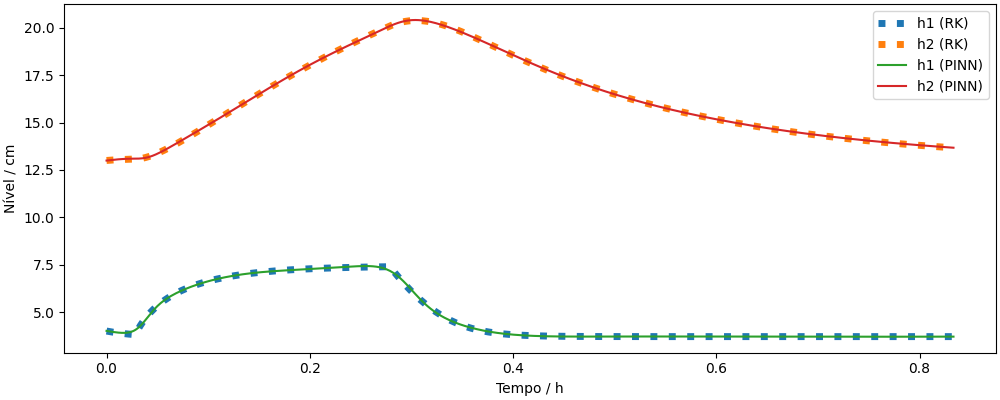
\includegraphics[width=1\textwidth]{pinn-result.png}
    \caption{Comparação entre as previsões da PINN e o método numérico (RK45).}
  \end{figure}
\end{frame}

\begin{frame}{Comparação de Tempos de Execução}
  \begin{figure}
    \centering
    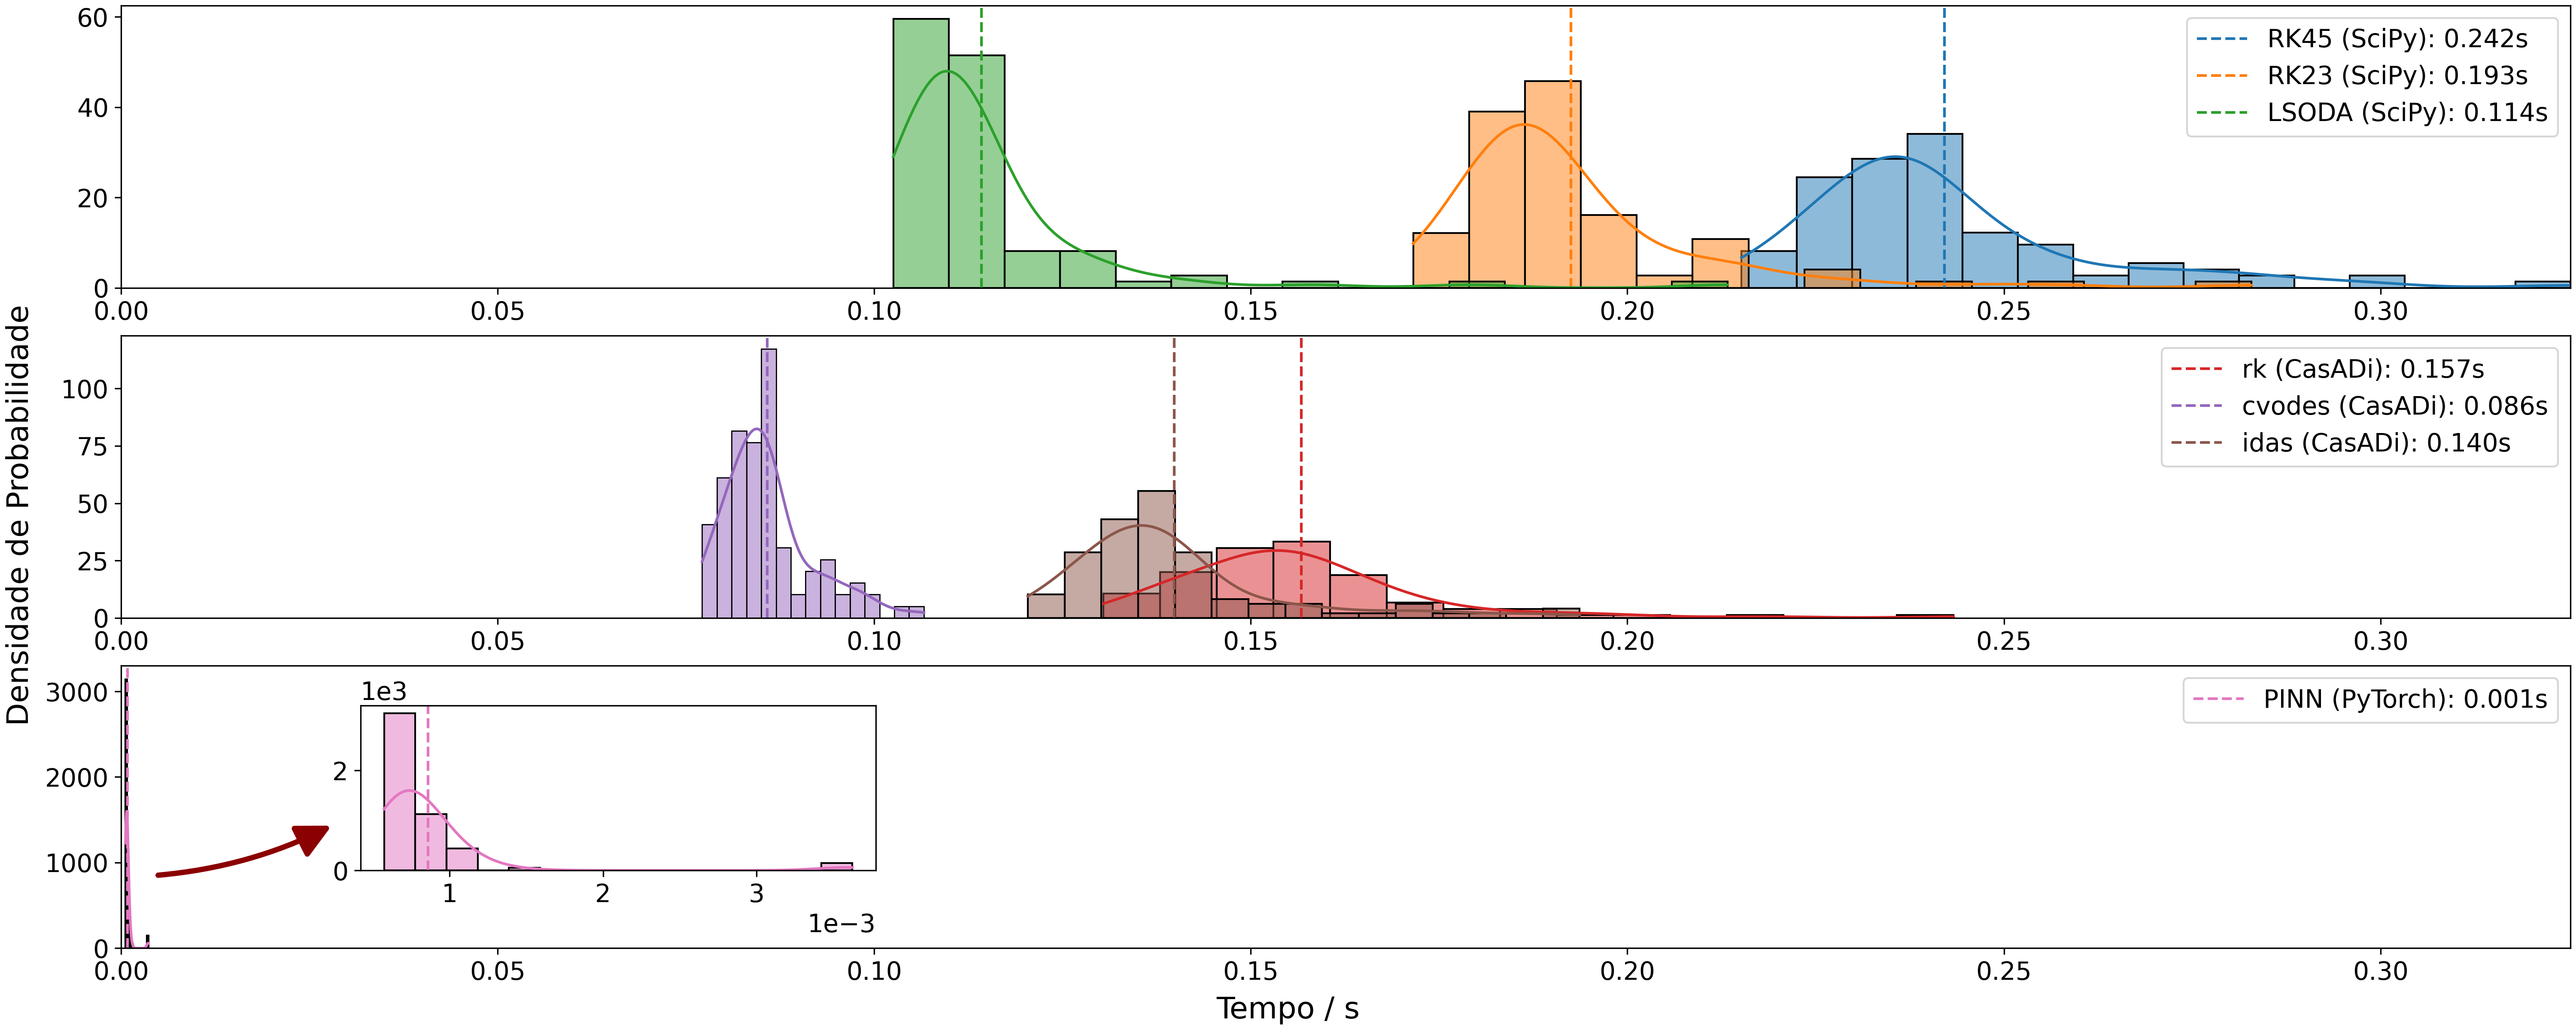
\includegraphics[width=\textwidth]{pinn-benchmark.png}
    \caption{Densidade de probabilidade dos tempos de execução dos métodos avaliados. Cada método foi executado 100 vezes; as linhas tracejadas indicam os tempos médios.}
  \end{figure}
\end{frame}
